\documentclass[12pt]{report} 
\usepackage{amsmath,amssymb} 
\usepackage[a4paper,margin=1in]{geometry} 

\usepackage{graphicx}
\usepackage{svg}

\usepackage{tikz}

 \begin{document} 
  \begin{figure}[htbp] \centering 
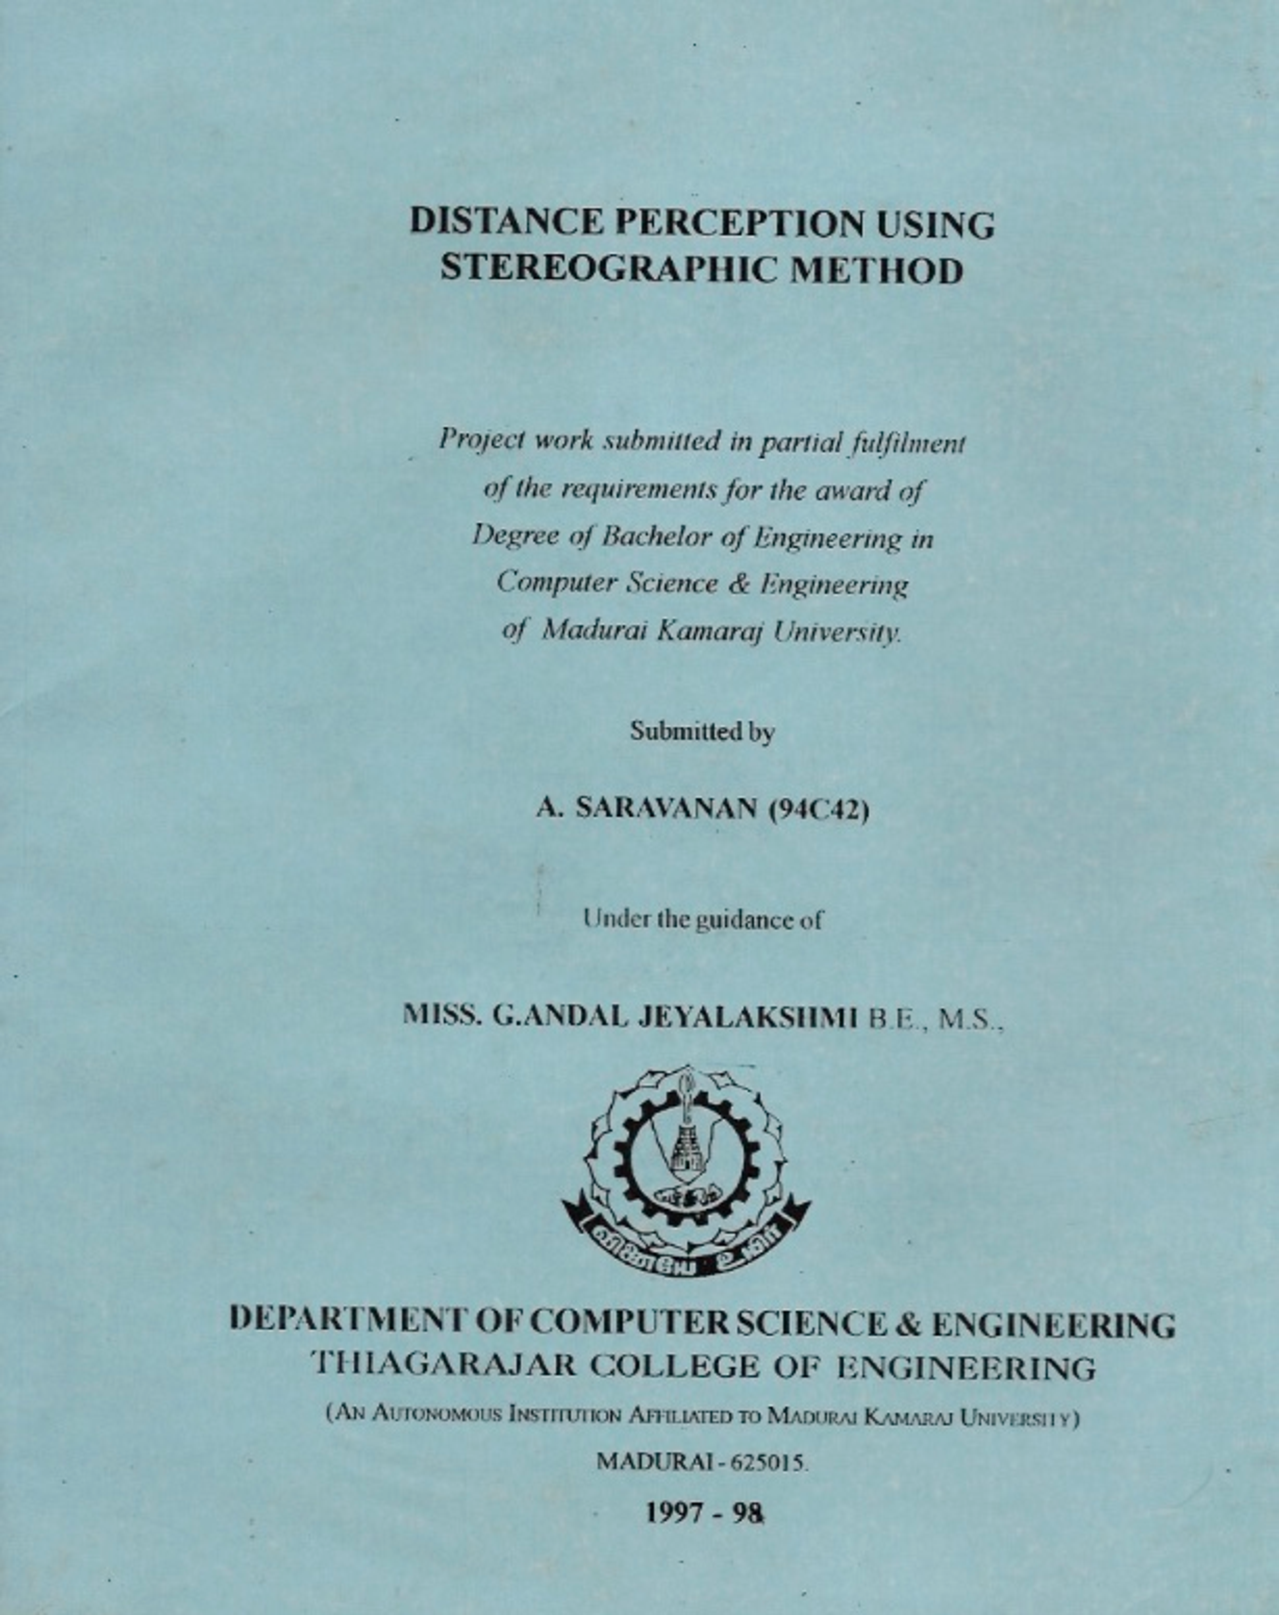
\includegraphics[width=0.8\textwidth]{title-page.pdf}
\end{figure}
 \begin{figure}[htbp] \centering 
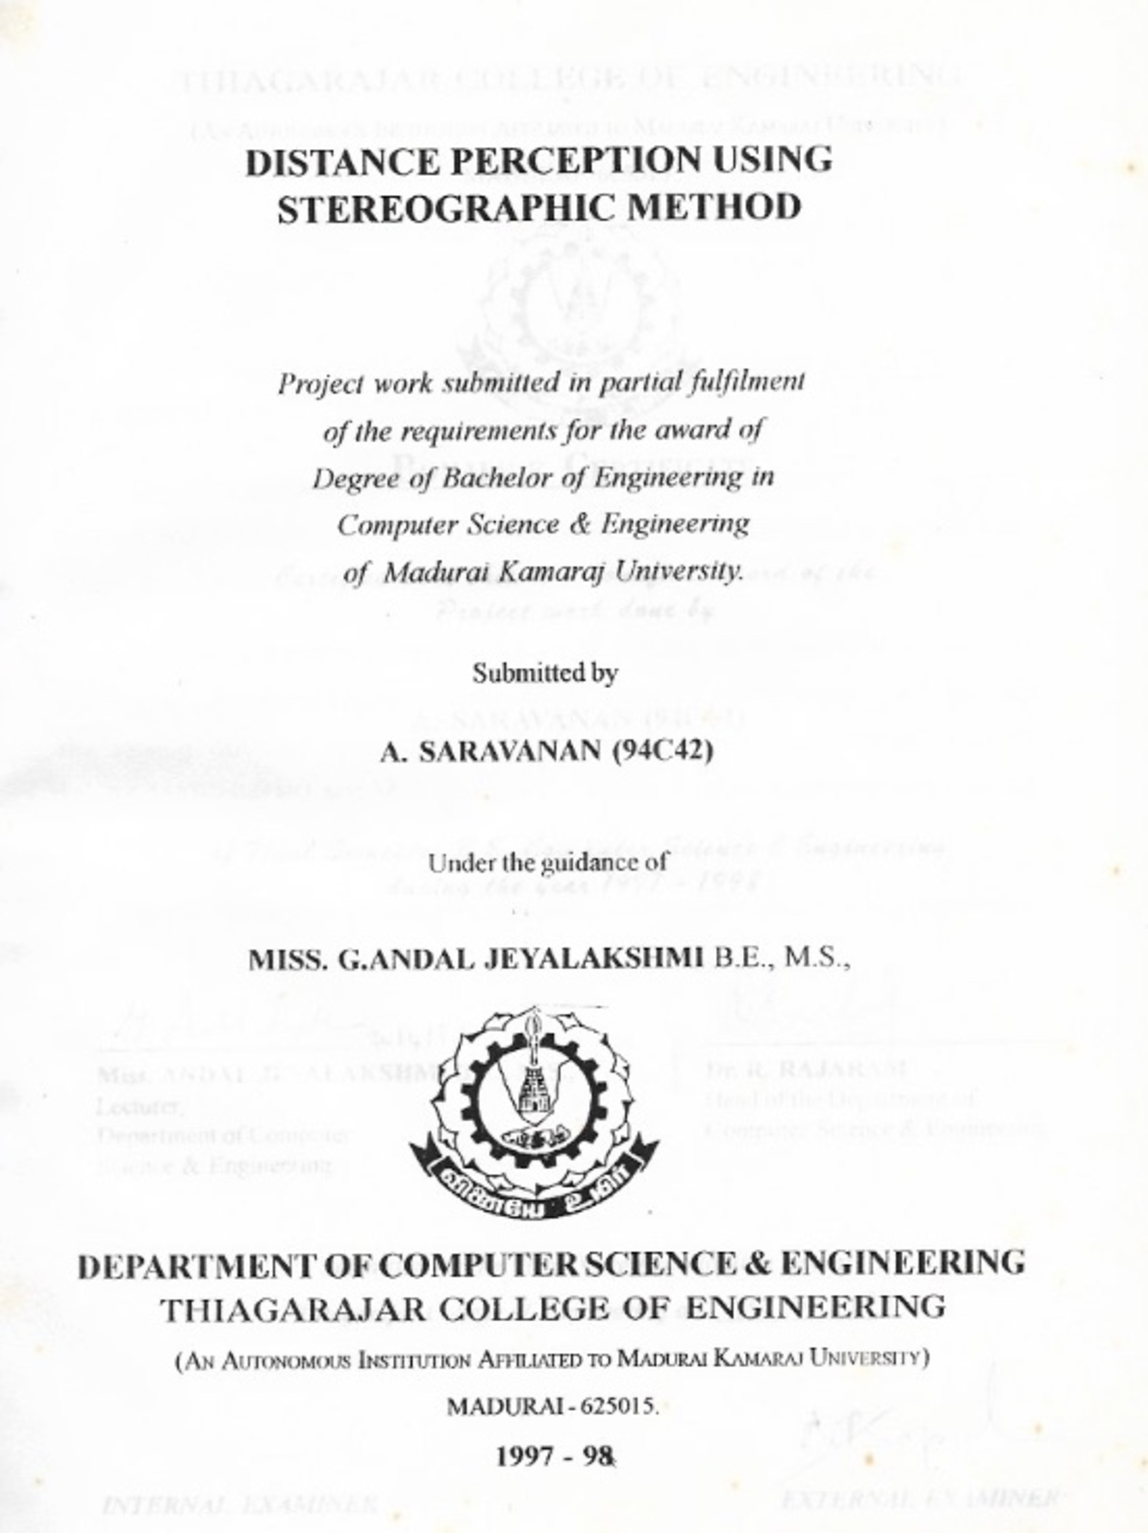
\includegraphics[width=0.8\textwidth]{first-page.pdf}
\end{figure}
 \begin{figure}[htbp] \centering 
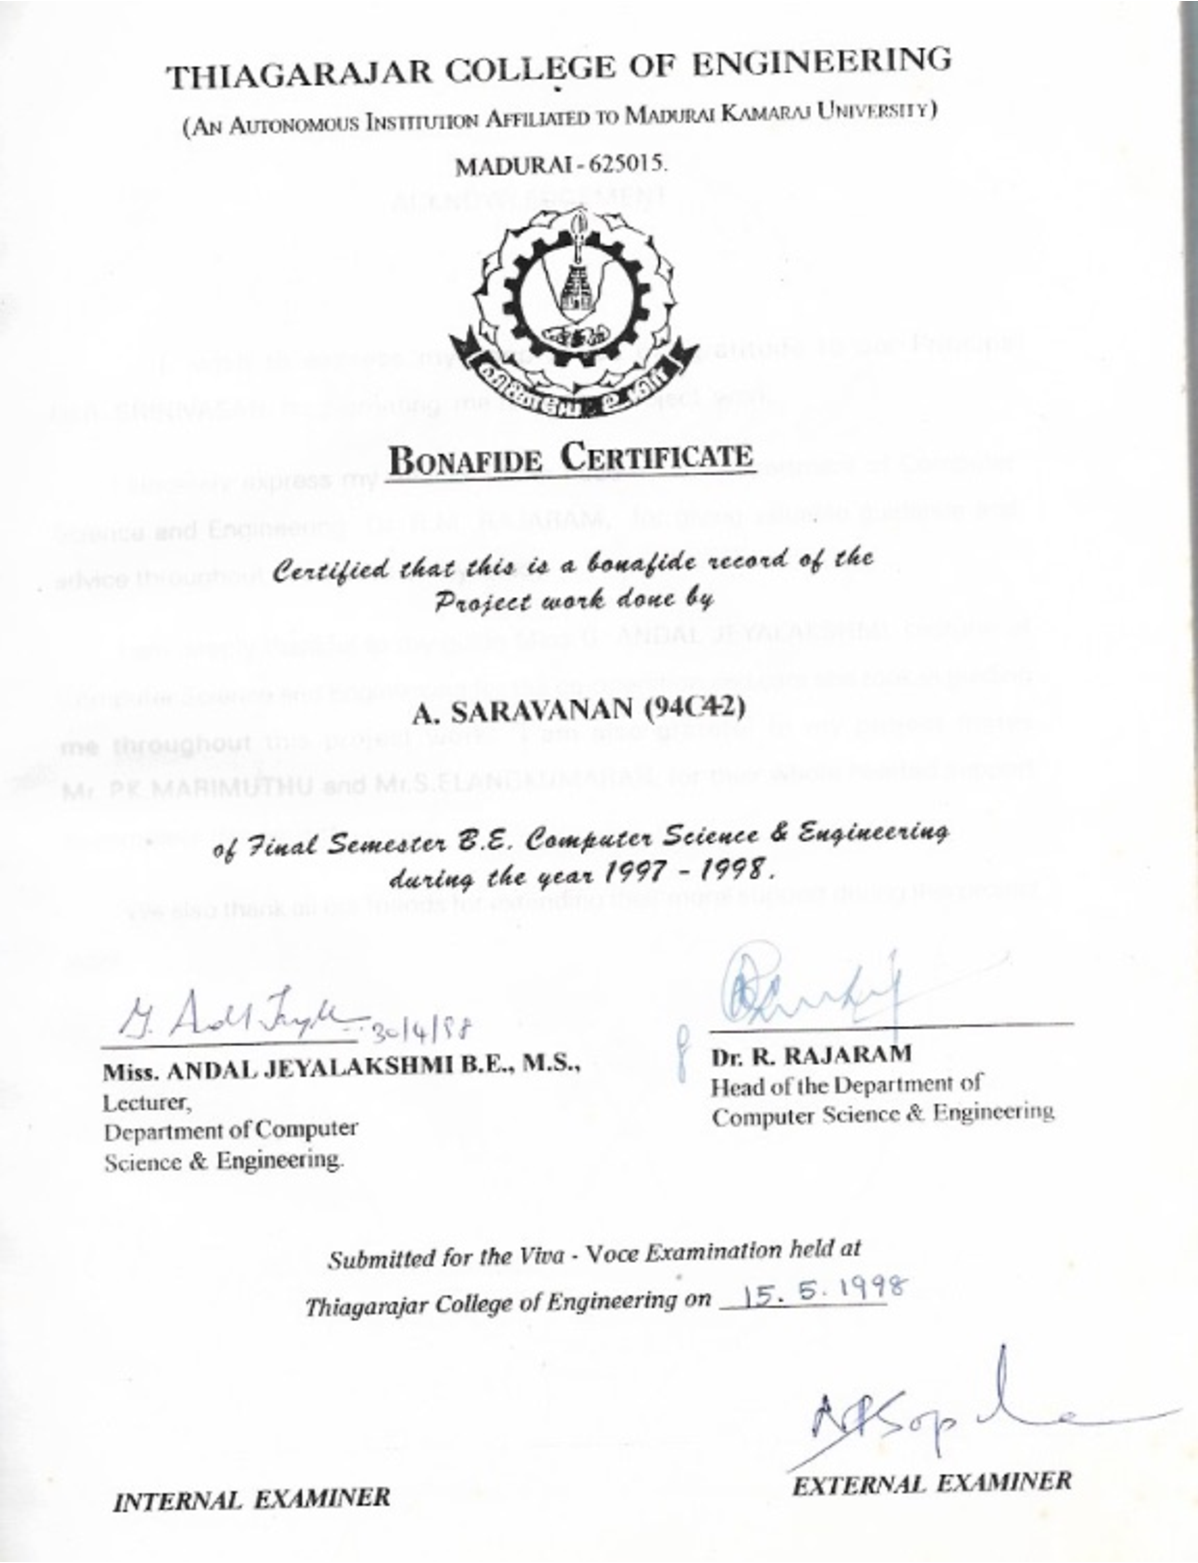
\includegraphics[width=0.8\textwidth]{sign-page.pdf}
\end{figure}
 
 \chapter*{ACKNOWLEDGEMENT} \addcontentsline{toc}{chapter}{ACKNOWLEDGEMENT} I wish to express my deep sense of gratitude to our Principal, Dr.\ R.\ Srinivasan, for permitting me to undertake this project work. \vspace{0.3cm} I sincerely express my thanks to our Head of the Department of Computer Science and Engineering, Dr.\ R.\ M.\ Rajaram, for providing valuable guidance and advice throughout the course of my study. \vspace{0.3cm} I am deeply thankful to my guide, Miss G.\ Andal Jeyalakshmi, Lecturer in Computer Science and Engineering, for the cooperation and care taken in guiding me throughout this project work. \vspace{0.3cm} I am also grateful to my project mates, Mr.\ P.\ K.\ Marimuthu and Mr.\ S.\ Elangkumaran, for their wholehearted support in completing this project. \vspace{0.3cm} I also thank all my friends for extending their moral support during this project work.
 \begin{figure}[htbp] \centering 

\includegraphics[width=0.8\textwidth]{dedication.pdf}
\end{figure}

\chapter{SYNOPSIS} Our project is to make the machine perceive the exact location of a point in the real world. This is the replication of visual capabilities of a human being on a computer. This is possible by first taking two photographs of a situation in the real world from two different views, for which the distances between those places are known. The images were stored as Bitmap files and analysed for the occurrence of a specific point. After finding that point, the system adopts a mathematical model and calculates the distance of that point from the camera. The mathematical model connects the image points and the real point in the real world, resulting in a geometrical figure by which the system is able to distinguish a point. This shows that concepts related to sense-data can be brought to machines by using simple but elegant mathematical formalism.

 \chapter{SYSTEM STUDY} 
\section{Historical Introduction} 
In those days before Christ, people were very interested in knowing how far the mystical celestial bodies were from the Earth. This was first done by the Greeks using the stereographic method. They observed the relationship between the disparity of an object when viewed from the left and right eye and its distance. They used the same technique for finding the distance of space objects by observing them from two different locations. During observation, measurements such as angles were taken, from which the distance was subsequently calculated. Later, in the seventeenth century, the philosopher Leibnitz introduced \textit{Monadology}, which describes how the brain manipulates monads. Monads were considered the mental equivalents of real-world objects. In the twentieth century, the mathematician and philosopher Bertrand Russell extended the concept of Monadology and explained how the brain analyses monads and combines them to determine the distance of an object. However, monads do not possess common elements. Consequently, a difficulty arises, leading Russell to conclude that Monadology alone is insufficient. Russell therefore gave greater importance to sense-data rather than monads. Sensibilia became the key to understanding distance perception. Since sensibilia contain common elements, the brain is able to identify these common elements and thereby perceive distance. This idea provided the basis for replicating the above process in machines. 
\section{Introduction to Our System} A computer has no direct receiver for sensibilia. Therefore, cameras have been used as the equivalent of eyes. By using cameras as eyes, algorithms as the equivalent of the thought process of the brain, and an appropriate mathematical model, machine vision can be achieved. However, because of limitations in present-day systems, the work presented here is on a relatively small scale.
 \subsection*{The Method} Two photographs of a real-world scene are taken from two different locations. The separation between the cameras is known and is measured as the distance between the centres of the lenses of the two cameras. Throughout this report, the distance between cameras implicitly refers to the distance between the centres of their lenses. The separation of the cameras is only in the horizontal direction. The photographs are stored as bitmap files. Information from these photographs is then transferred to two arrays. In a literal sense, these arrays are the machine equivalents of sensibilia. The two arrays are then convolved in order to locate a particular point. This is accomplished by searching for a corresponding point in both arrays. The position of the point in each photograph can then be described using Cartesian coordinates, with the centre taken as the origin. Using these coordinates, a simple geometric structure can be constructed that contains all the information required. Thus, even though most of the operations are performed manually, the system is capable of perceiving distance in a literal sense. 
 \section{About Bitmap Files} The two photographs are scanned using a scanner and stored as bitmap (BMP) files. Bitmap files contain mapped pixel information corresponding to points in the scanned photograph. A bitmap file is an uncompressed file. Since this file represents the machine equivalent of sensibilia, it must be analysed in order to obtain the required information. A bitmap file contains three header structures. The first header structure contains a variable that identifies whether the file is a BMP file. It also contains a variable indicating the location of the pixel information within the file. A detailed description of all variables in these header structures is beyond the scope of this work. The second header contains several variables. Of particular interest are: 
 \begin{itemize} 
 \item \texttt{biWidth} \item \texttt{biHeight} \item \texttt{biXPelsPerMeter} \item \texttt{biYPelsPerMeter} \item \texttt{biBitCount} \end{itemize} The variable \texttt{biBitCount} indicates the number of bits used to represent a particular colour. The variables \texttt{biWidth} and \texttt{biHeight} specify the width and height of the image in pixels. The remaining two variables specify the number of pixels per metre in the horizontal and vertical directions. The third header structure specifies the proportions of red, green, and blue required to represent a particular colour. One structure is used for each colour. Therefore, the structure is repeated as many times as the number of colours used in the file. The number of colours can be determined from the second-header variable \texttt{biClrUsed}. These repeated structures form a colour table. When the data area is accessed, it provides a pointer to an entry within this colour table. All information can be accessed through the available pointers. The data is transferred into two-dimensional arrays. Information from the other photograph is similarly transferred into another array. These arrays are then processed to obtain the required information. The manner in which this processing is performed is explained in the subsequent chapters.
 
 \chapter{MATHEMATICAL MODEL} 
 \section{Introduction} 
 Cameras usually capture objects upside down and reversed from left to right, as is well known. In this chapter, all discussions are based on negatives. However, in the subsequent chapters, the discussion may refer either to negatives or to photographs because only photographs are stored and processed in the computer, and a photograph is the reflection of an object. Referring to Fig.~3.1, it can be seen that point $P$ is captured by both cameras, and the corresponding image of the point can be located by two sets of image coordinates $(x_l,y_l)$ and $(x_r,y_r)$. Here, the suffixes $l$ and $r$ denote the left and right negatives respectively. In the diagram and throughout the following discussion, we adopt the convention that the observer is facing the camera from the real world. Consequently, for a person viewing the real world from behind the camera, the left side for the observer corresponds to the right side of that person.
  \section{Calculating $x$ and $z$} To perceive the location of any point, three coordinates $x$, $y$, and $z$ are required. These coordinates are determined using the mathematical model described below. Figure~3.2 represents the top view of Fig.~3.1. In this figure, points $A$ and $B$ denote the centres of the left and right cameras respectively. 
  
  There is the distance between the camera lens centre and negative's centre. 
\vspace{0.5cm} And the known distance is denoted by $d$. \vspace{0.5cm} With point's image co-ordinates following calculation were made. \begin{equation} \theta_{1} = \tan^{-1} \left| \frac{f}{x_{l}} \right| \tag{3.1} \end{equation} \begin{equation} \theta_{2} = \tan^{-1} \left| \frac{f}{x_{r}} \right| \tag{3.2} \end{equation} We know that \begin{align} \alpha &= \theta_{1} \tag{3.3}\\[6pt] \beta &= \theta_{2} \tag{3.4}\\[6pt] \gamma &= 180^\circ - (\alpha + \beta) \tag{3.5} \end{align} For any triangle like $\triangle ABC$ here, the equality (3.6) is true. \begin{equation} \frac{\sin\alpha}{a} = \frac{\sin\beta}{b} = \frac{\sin\gamma}{d} \tag{3.6} \end{equation} $a$, $b$ and $d$ were sides opposite to angle $\alpha$, $\beta$ and $\gamma$. \vspace{0.5cm} For the proof of (3.6) see Appendix B and C. \vspace{0.5cm} We know angles $\alpha$, $\beta$ and $\gamma$ and side $d$ so other two sides were calculated as \begin{equation} a = \frac{\sin\alpha}{\sin\gamma} \times d \tag{3.7} \end{equation}


\begin{equation} a = \frac{\sin\beta}{\sin\gamma} \times d \tag{3.8} \end{equation} The real coordinates $x$, $y$, $z$ were calculated as below. Here we conventionally take the centre of lens as the origin. \vspace{0.5cm} As told already the cameras were separated in $x$-direction. So two real coordinates set can be obtained but on both, $y$ and $z$ will be the same but $x$. So two $x$ were calculated \begin{align} Lx &= b\cos\alpha \tag{3.9}\\[6pt] Rx &= a\cos\beta \tag{3.10} \end{align} $z$ can be calculated either as \begin{align} z &= \sqrt{b^{2} - (Lx)^{2}} \qquad \text{or as} \tag{3.11}\\[6pt] z &= \sqrt{a^{2} - (Rx)^{2}} \tag{3.12} \end{align} Theoritically both $z$ values must be same. But due to manual errors incurred during shooting picture it may vary with negligible amount. \vspace{1cm} \noindent \textbf{3.3. Calculating Y.} \vspace{0.5cm} Fig. 3.3 is the sideview of Fig. 3.1. $y_l$ and $y_r$ were two image coordinates. With the help of one of these real $y$ can be calculated. As said above the calculation by taking one $y$ won't match with by taking other $y$. This is because of manual error as said above.

\section{Calculating $Y$} Now, \begin{equation} \theta_{3} = \tan^{-1} \left| \frac{y_l}{f} \right| \tag{3.13} \end{equation} We know all three coordinates of that point now. With this, we can perform the task of locating that point. As stated in the introduction, all measurements were calculated only from the images after the observation was completed. We can now determine the angle at which the point is located and its straight-line distance from the lens. Thus the slant distances for the left and right cameras are given by \begin{equation} \text{s-d-l} = \sqrt{(Lx)^2 + Y^2 + Z^2} \tag{3.14} \end{equation} \begin{equation} \text{s-d-r} = \sqrt{(Rx)^2 + Y^2 + Z^2} \tag{3.15} \end{equation} The above equations are theoretical. The method used to computerize these calculations is explained in the subsequent chapters.

\begin{figure}[htbp] \centering 
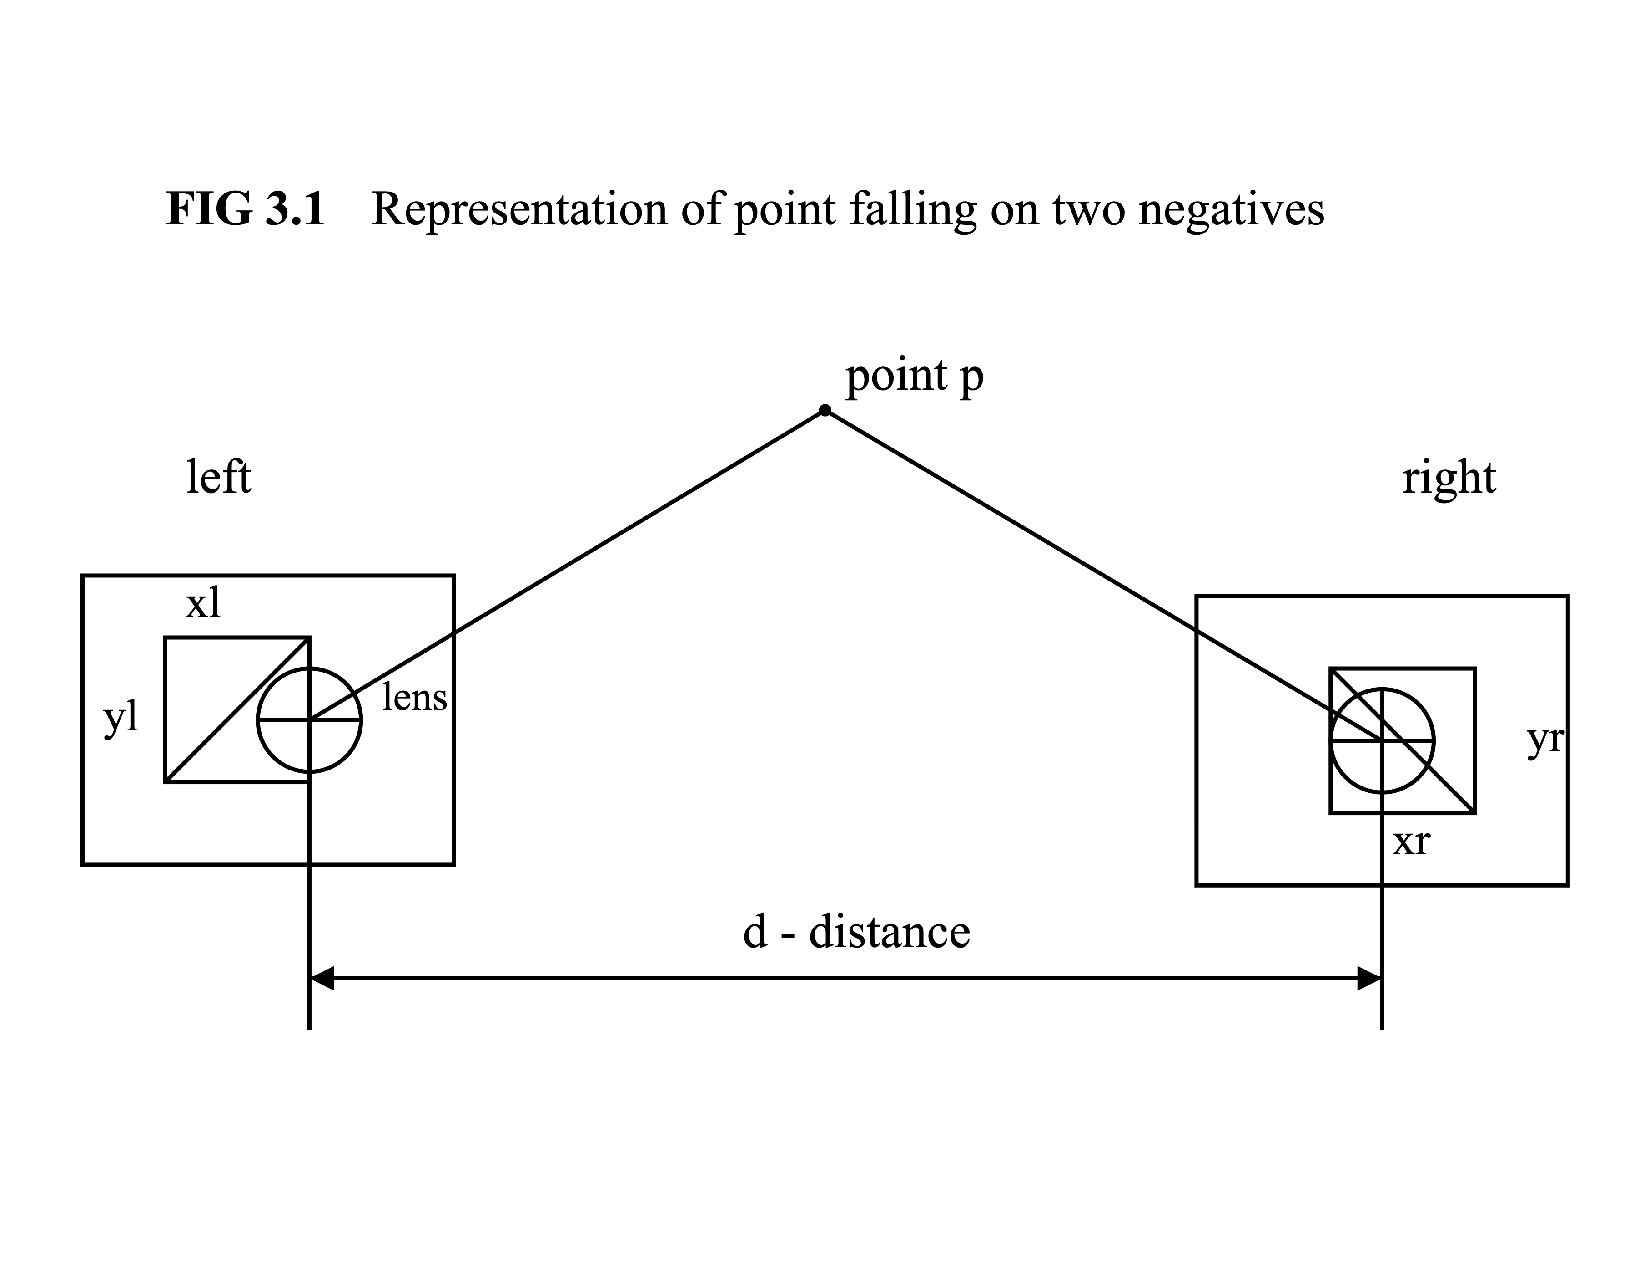
\includegraphics[width=0.8\textwidth]{fig31.pdf}
\caption{Representation of point falling on two negatives} 
\label{fig:stereo_negatives} 
\end{figure}

\begin{figure}[htbp] \centering 
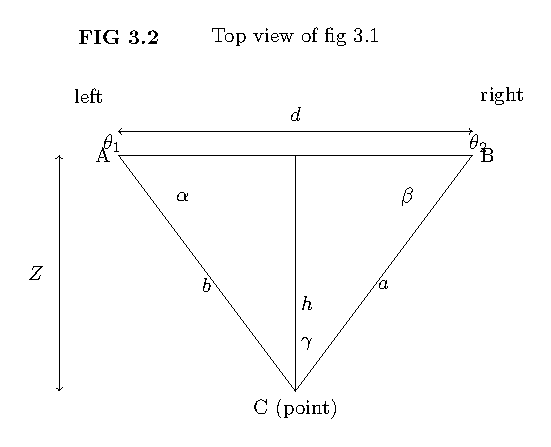
\includegraphics[width=0.8\textwidth]{figure32.pdf}
\caption{Representation of point falling on two negatives} 
\label{fig:stereo_negatives} 
\end{figure}

\begin{figure}[htbp] \centering 
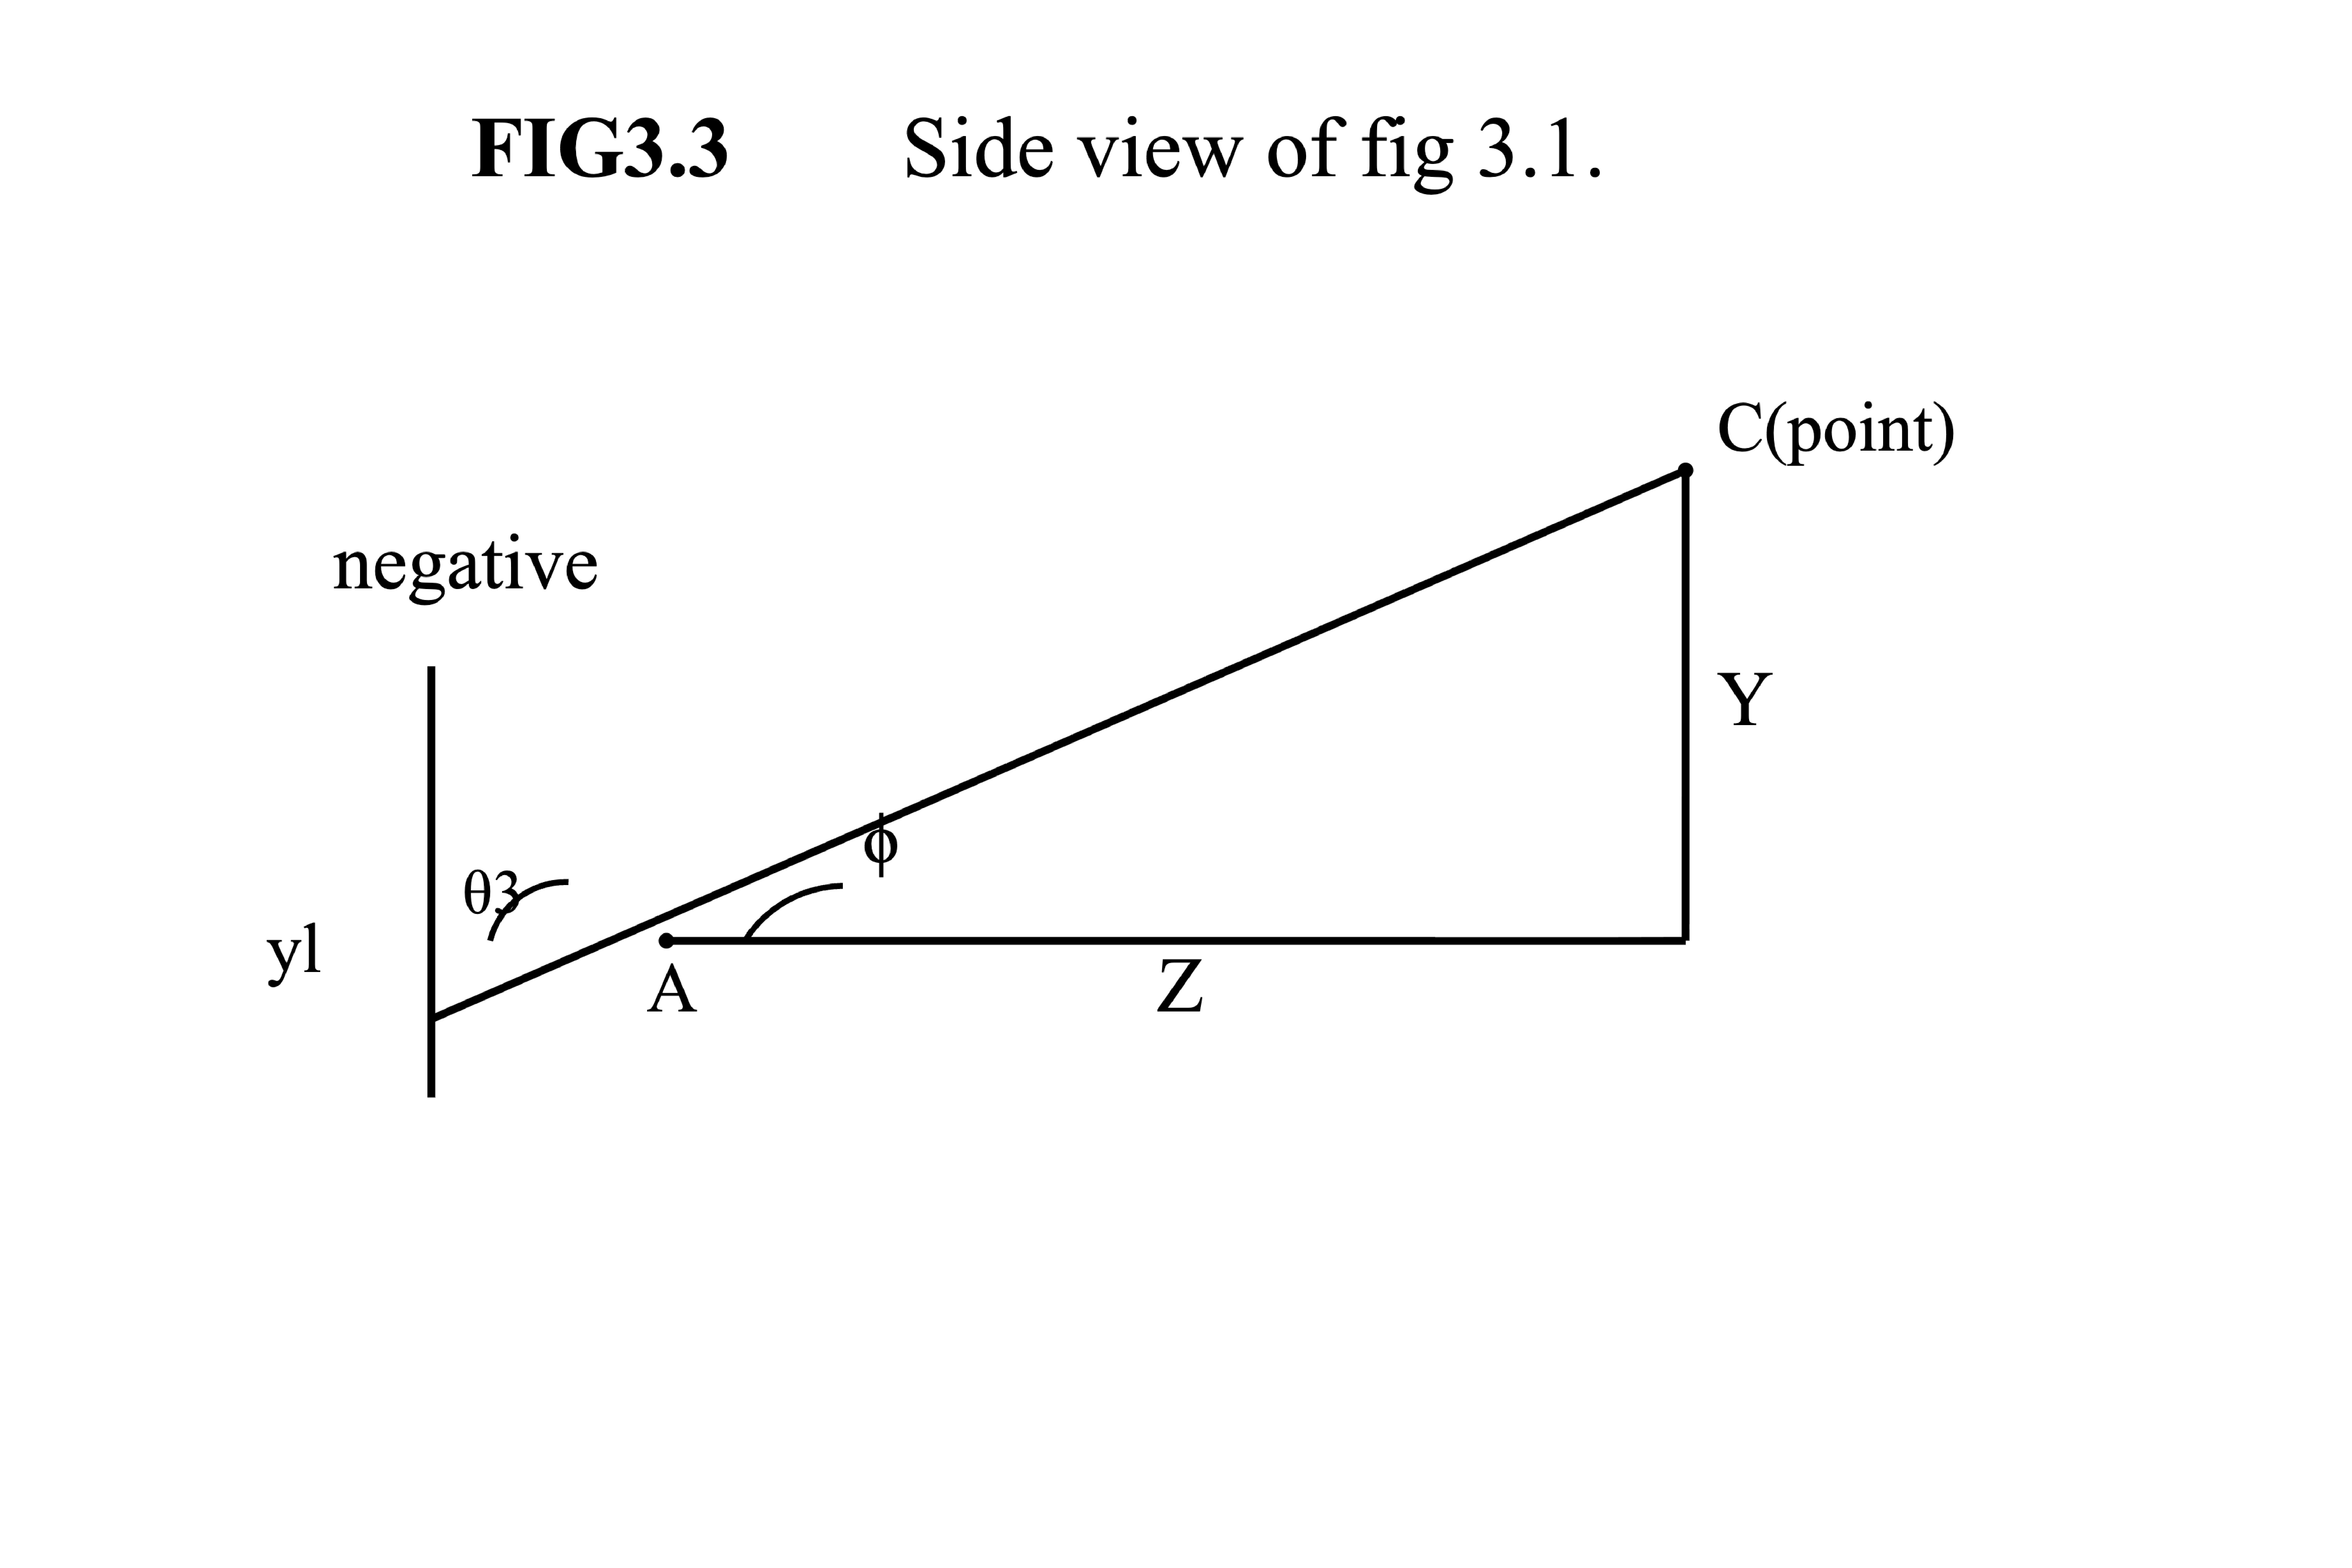
\includegraphics[width=0.8\textwidth]{figure33.pdf}
\caption{Representation of point falling on two negatives} 
\label{fig:stereo_negatives} 
\end{figure}

\chapter{SYSTEM DESIGN \& FLOW CHART} The photographs were scanned using a black-and-white scanner and the files were stored as BMP files. The steps followed in the processing of the images are as follows: \begin{enumerate} \item Access the BMP file header structures to determine the characteristics of the photograph and obtain information about all pixels. \item Create an array having the same size as the BMP file and transfer all pixel information to that array. The above two operations are performed twice, once for the left photograph and once for the right photograph. \item Search the left array for the occurrence of a point on the object for which the distance is to be determined. \item If the point is found, perform the same search on the right array. Otherwise, display an error message indicating that no valuable point is available and terminate the process. \item If a matching point is found in the right array, proceed to the next step. Otherwise, display an error message indicating that the photographs may be incorrect. \item Obtain the image coordinates from the array indices. \item Convert the image coordinates into equivalent negative coordinates for further calculations. \item Calculate the three-dimensional coordinates using $x_l$, $y_l$, $x_r$, and $y_r$. \item The computer now determines the position of the required point. \item Print the results. \end{enumerate} A detailed description of these steps is given in the next chapter.

\begin{figure}[htbp] \centering 
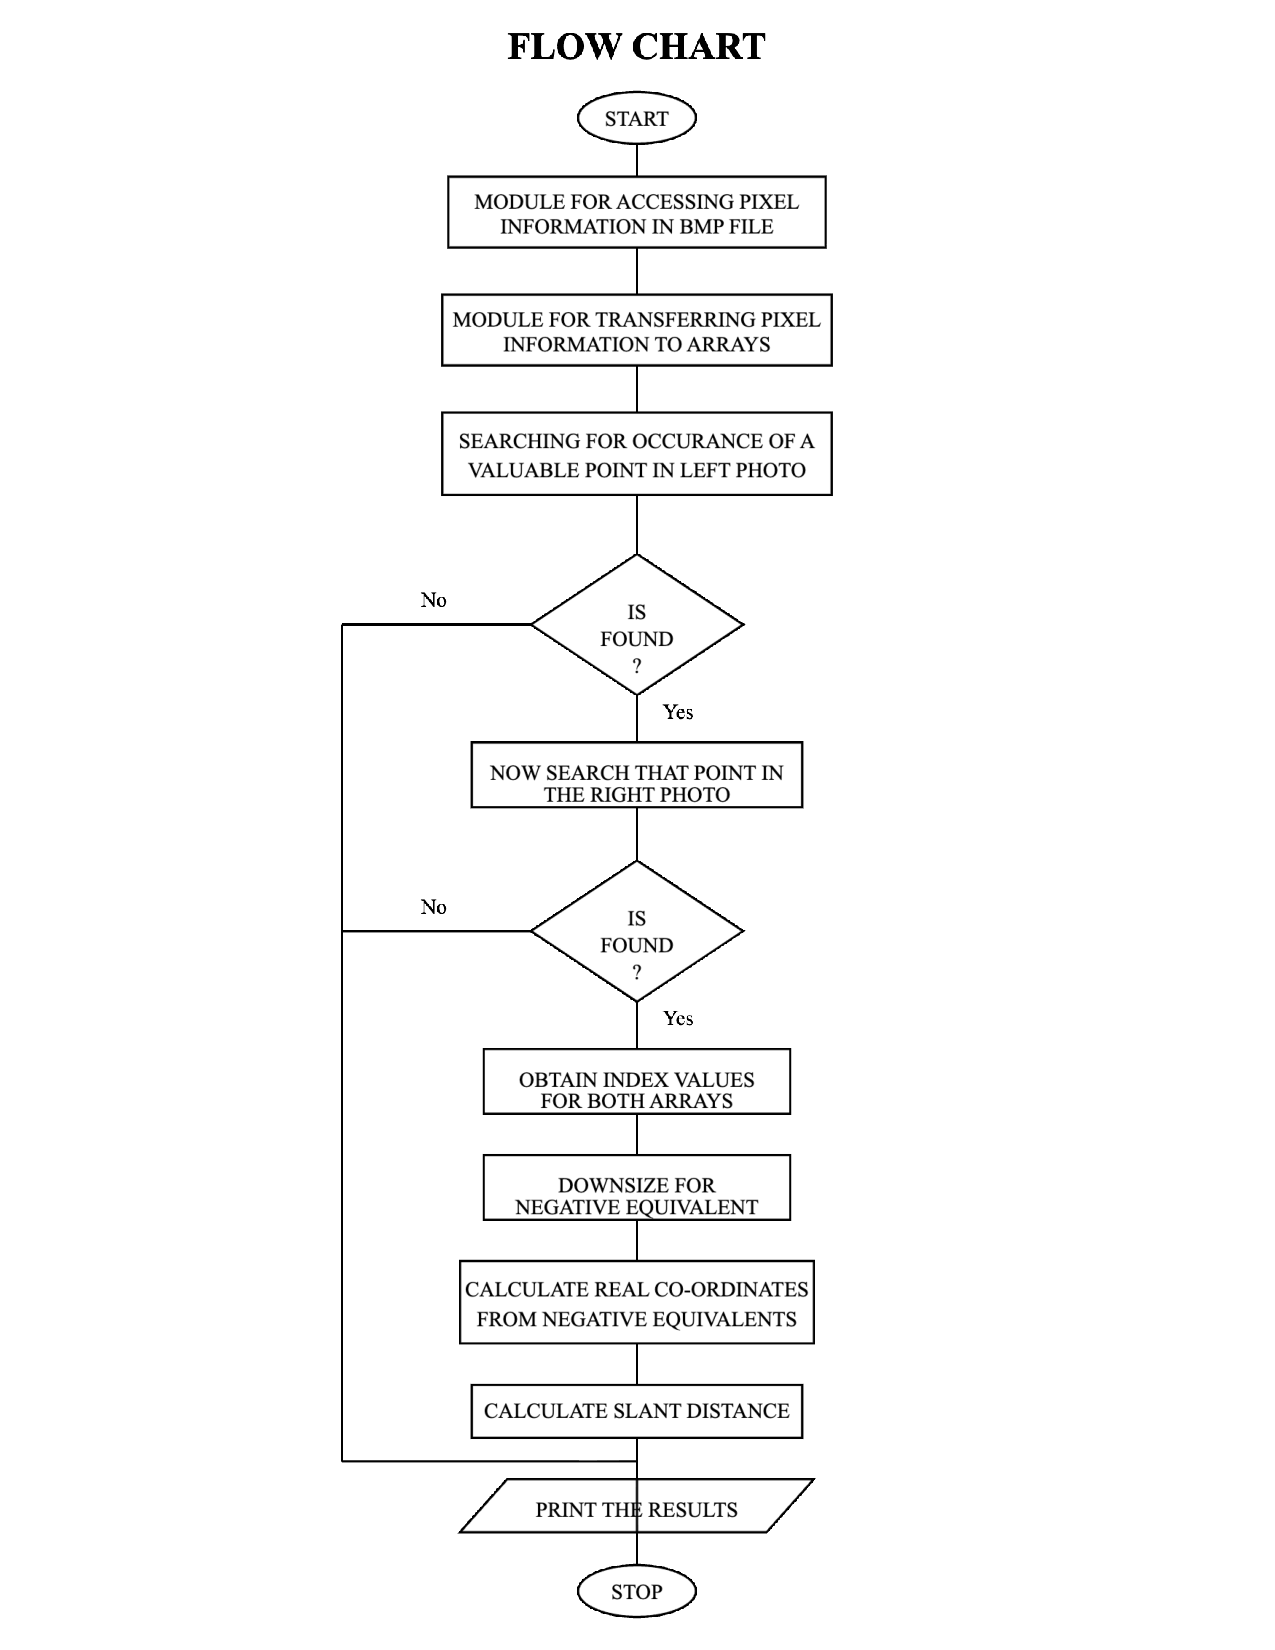
\includegraphics[width=0.8\textwidth]{flow-chart.pdf}
\caption{Representation of point falling on two negatives} 
\label{fig:stereo_negatives} 
\end{figure}


\chapter{IMPLEMENTATION} \section{Searching a Valuable Point} The valuable point may be defined differently in different contexts. We have used a black-and-white scanner. Therefore, discrimination and decision making based on minor variations may lead to uncertainty. Hence, we consider a very simple case in which a valuable point is defined as a point having a colour different from that of the background. The background colour can be assigned manually. When we observe Fig.~5.1, we can easily visualize that a point in side LR has a counterpart only in RR, and a point in RL has a counterpart only in LL. This reduces the overall search process to an optimized search. If a point is not found in either pair, a third alternative is adopted. That is, searching in the LL and RR sides. The figure describes the situation for negatives, whereas the array is the photo-equivalent and a $180^\circ$ rotated image of the negative. 
Therefore, the optimized search on the array is as follows: 
\begin{enumerate}
\item LL, then RL 
\item RR, then LR 
\item 
If not found by (a) or (b), then LR and RL 
\end{enumerate} 
Another optimization is that when a valuable point is found in one array, its counterpart can theoretically be found in the same row without searching any other row. However, due to manual errors, an allowance is provided. Accordingly, the algorithm searches 4 to 6 rows above and below the row in which the corresponding point is found in the other array. 

\subsection{DOWNSIZING AND CALCULATION} After a valuable point is found, its coordinates are obtained. However, the picture is enlarged and the model proposed is based on negative coordinates. Therefore, these coordinates must be reduced to negative size. Let $X_b$ and $Y_b$ be the coordinates corresponding to the size of the BMP file. We know the BMP file's width, height, and converting ratios (\texttt{xpelspermeter} and \texttt{ypelspermeter}). Using these values, we convert $X_b$, $Y_b$, width, and height from number of pixels into metres or millimetres, resulting in $x_m$, $y_m$, width$_m$, and height$_m$. \vspace{0.5cm} So, \begin{equation} X_m = \frac{1}{\text{Xpelspermeter}} \times X_b \ \text{meter} \tag{5.1} \end{equation} \begin{equation} Y_m = \frac{1}{\text{Ypelspermeter}} \times Y_b \ \text{meter} \tag{5.2} \end{equation} \begin{equation} \text{Width}_m = \frac{\text{width}} {\text{Xpelspermeter}} \ \text{meter} \tag{5.3} \end{equation} \begin{equation} \text{Height}_m = \frac{\text{height}} {\text{Ypelspermeter}} \ \text{meter} \tag{5.4} \end{equation} From these metric-converted variables, we obtain $x_l$, $y_l$, $x_r$, and $y_r$.

The camera used in this project has a negative size of 35\,mm $\times$ 24\,mm. Let these dimensions be denoted by $w_n$ and $h_n$ respectively. \vspace{0.5cm} So, \begin{equation} x_l = \frac{x_m}{\text{width}_m} \times \frac{h_n}{1000} \ \text{meter} \tag{5.5} \end{equation} \begin{equation} y_l = \frac{y_m}{\text{height}_m} \times \frac{w_n}{1000} \ \text{meter} \tag{5.6} \end{equation} Similarly, we can determine $x_l$, $y_l$ and $x_r$, $y_r$. Using these values, the real-world coordinates $x$, $y$, and $z$ can be calculated from Equations (3.1) to (3.12). \vspace{0.5cm} Thus, with the coordinates $x$, $y$, and $z$, our initial goal of enabling a computer to perceive a scene through a camera is achieved, at least in a primitive form.

The camera we have used has negative size as $35\,\mathrm{mm}\times24\,\mathrm{mm}$. We call it $w_n$ and $h_n$. \vspace{0.5cm} So \begin{equation} x_l = \frac{x_m}{\mathrm{width}_m} \times \frac{h_n}{1000} \ \mathrm{meter} \tag{5.5} \end{equation} \begin{equation} y_l = \frac{y_m}{\mathrm{height}_m} \times \frac{w_n}{1000} \ \mathrm{meter} \tag{5.6} \end{equation} Similarly we can find $x_l$, $y_l$ and $x_r$, $y_r$. We can determine real co-ordinates $x$, $y$, $z$ using formulae (3.1) to (3.12). \vspace{0.5cm} Thus, with $x$, $y$, and $z$, our initial goal of seeing by computer using a camera is achieved primitively.


\begin{figure}[htbp] \centering 
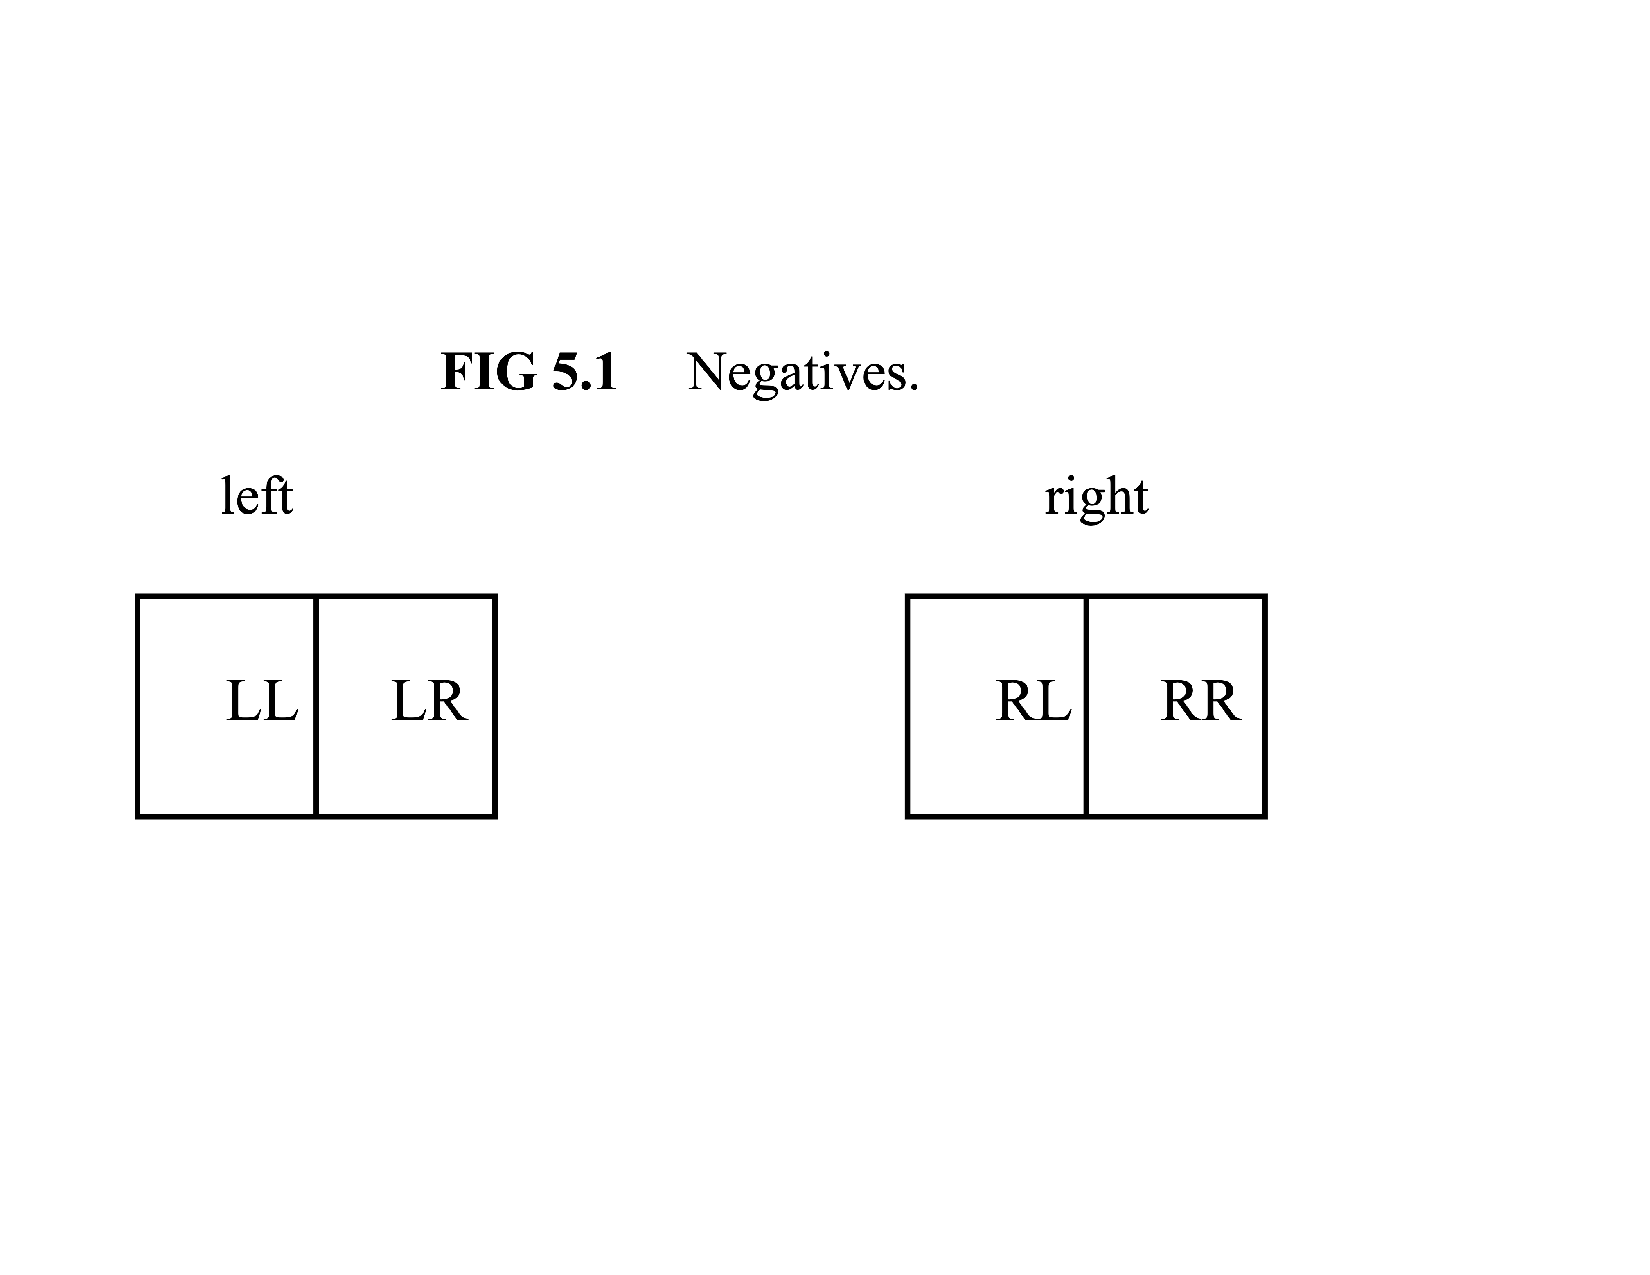
\includegraphics[width=0.8\textwidth]{negative-view.pdf}
\caption{Negative View} 
\label{fig:stereo_negatives} 
\end{figure}




\chapter{APPLICATIONS} It is possible to speculate on future applications that may evolve if the concepts presented in this work are extended and put into wider practice. \begin{enumerate} \item Vision is a continuous process. Therefore, in the future, video information may be processed in parallel. This can be achieved through a video processor that continuously processes video information and interrupts the main processor whenever a particular object or event is recognized. \item This system is not intended for determining the exact distance of objects. For such purposes, many engineering devices, such as SONAR, are available. The proposed system determines distance only approximately and therefore exhibits an inherent degree of uncertainty, which is fuzzy in nature. Consequently, this approach is more suitable for building intelligent machines rather than highly precise machines. Human intelligence is characterized by uncertainty, multivaluedness, and indeterminacy. Therefore, when extended, this system may serve as a basis for introducing or imparting fuzzy logic through visual sense-data. \item Another promising approach from the field of dynamical systems is Neural Networks. Neural networks can be trained using visual data and can be developed to recognize human faces or other objects. Such systems could significantly reduce the tedious work involved in identifying criminals or specific individuals and could automate many of these recognition tasks. \end{enumerate}

\chapter{CONCLUSION} We have taken photographs of the real world and tested our mathematical model, which theoretically gave precise results. After theoretical verification, we computerized the manual calculations. This was done by first scanning the photographs using a black-and-white scanner and storing them as BMP files. The data was then transferred into arrays. Subsequently, we successfully carried out the crucial task of finding a valuable point from a large array containing several lakh elements. Due to the limitations of the available hardware, the images were kept as simple as possible and involved only a single object. Calculations were carried out on the selected point, and the desired result, namely the distance of the object from the cameras, was obtained. We hope that in the future our system can be extended to process complex images containing thousands of distinguishable colours.

\chapter{BIBLIOGRAPHY} \begin{enumerate} \item Russell, Bertrand, \textit{Mysticism and Logic}. Routledge \& Kegan Paul, London, 1917. \vspace{0.5cm} \item Winston, Patrick Henry, \textit{Artificial Intelligence}, 3rd Edition. Addison-Wesley, Reading, Massachusetts, 1992. \vspace{0.5cm} \item \textit{Windows API Bible}. Galgotia Publishers, New Delhi, 1991. \end{enumerate}

\appendix \chapter*{APPENDICES} \addcontentsline{toc}{chapter}{APPENDICES} \section*{APPENDIX A} \addcontentsline{toc}{section}{APPENDIX A} The geometry involved, if in $\triangle ABC$ $\beta$ becomes an obtuse angle. A similar approach can also be given if angle $\alpha$ becomes obtuse. \vspace{0.5cm} From Fig.~A.1 \begin{align} \theta_1 &= \tan^{-1}\left|\frac{f}{x_l}\right| \\ \theta_2 &= \tan^{-1}\left|\frac{f}{x_r}\right| \end{align} \begin{align} \alpha &= \theta_1 \\ \beta &= 180^\circ - \theta_2 \\ \gamma &= 180^\circ - (\alpha + \beta) \end{align} \begin{align} Lx &= b \cdot \cos(\alpha) \\ Rx &= a \cdot \cos(180^\circ-\beta) \end{align} \begin{align} z &= \sqrt{b^2-(Lx)^2} \qquad \text{or} \\ z &= \sqrt{a^2-(Rx)^2} \end{align}

\begin{figure}[htbp] \centering 
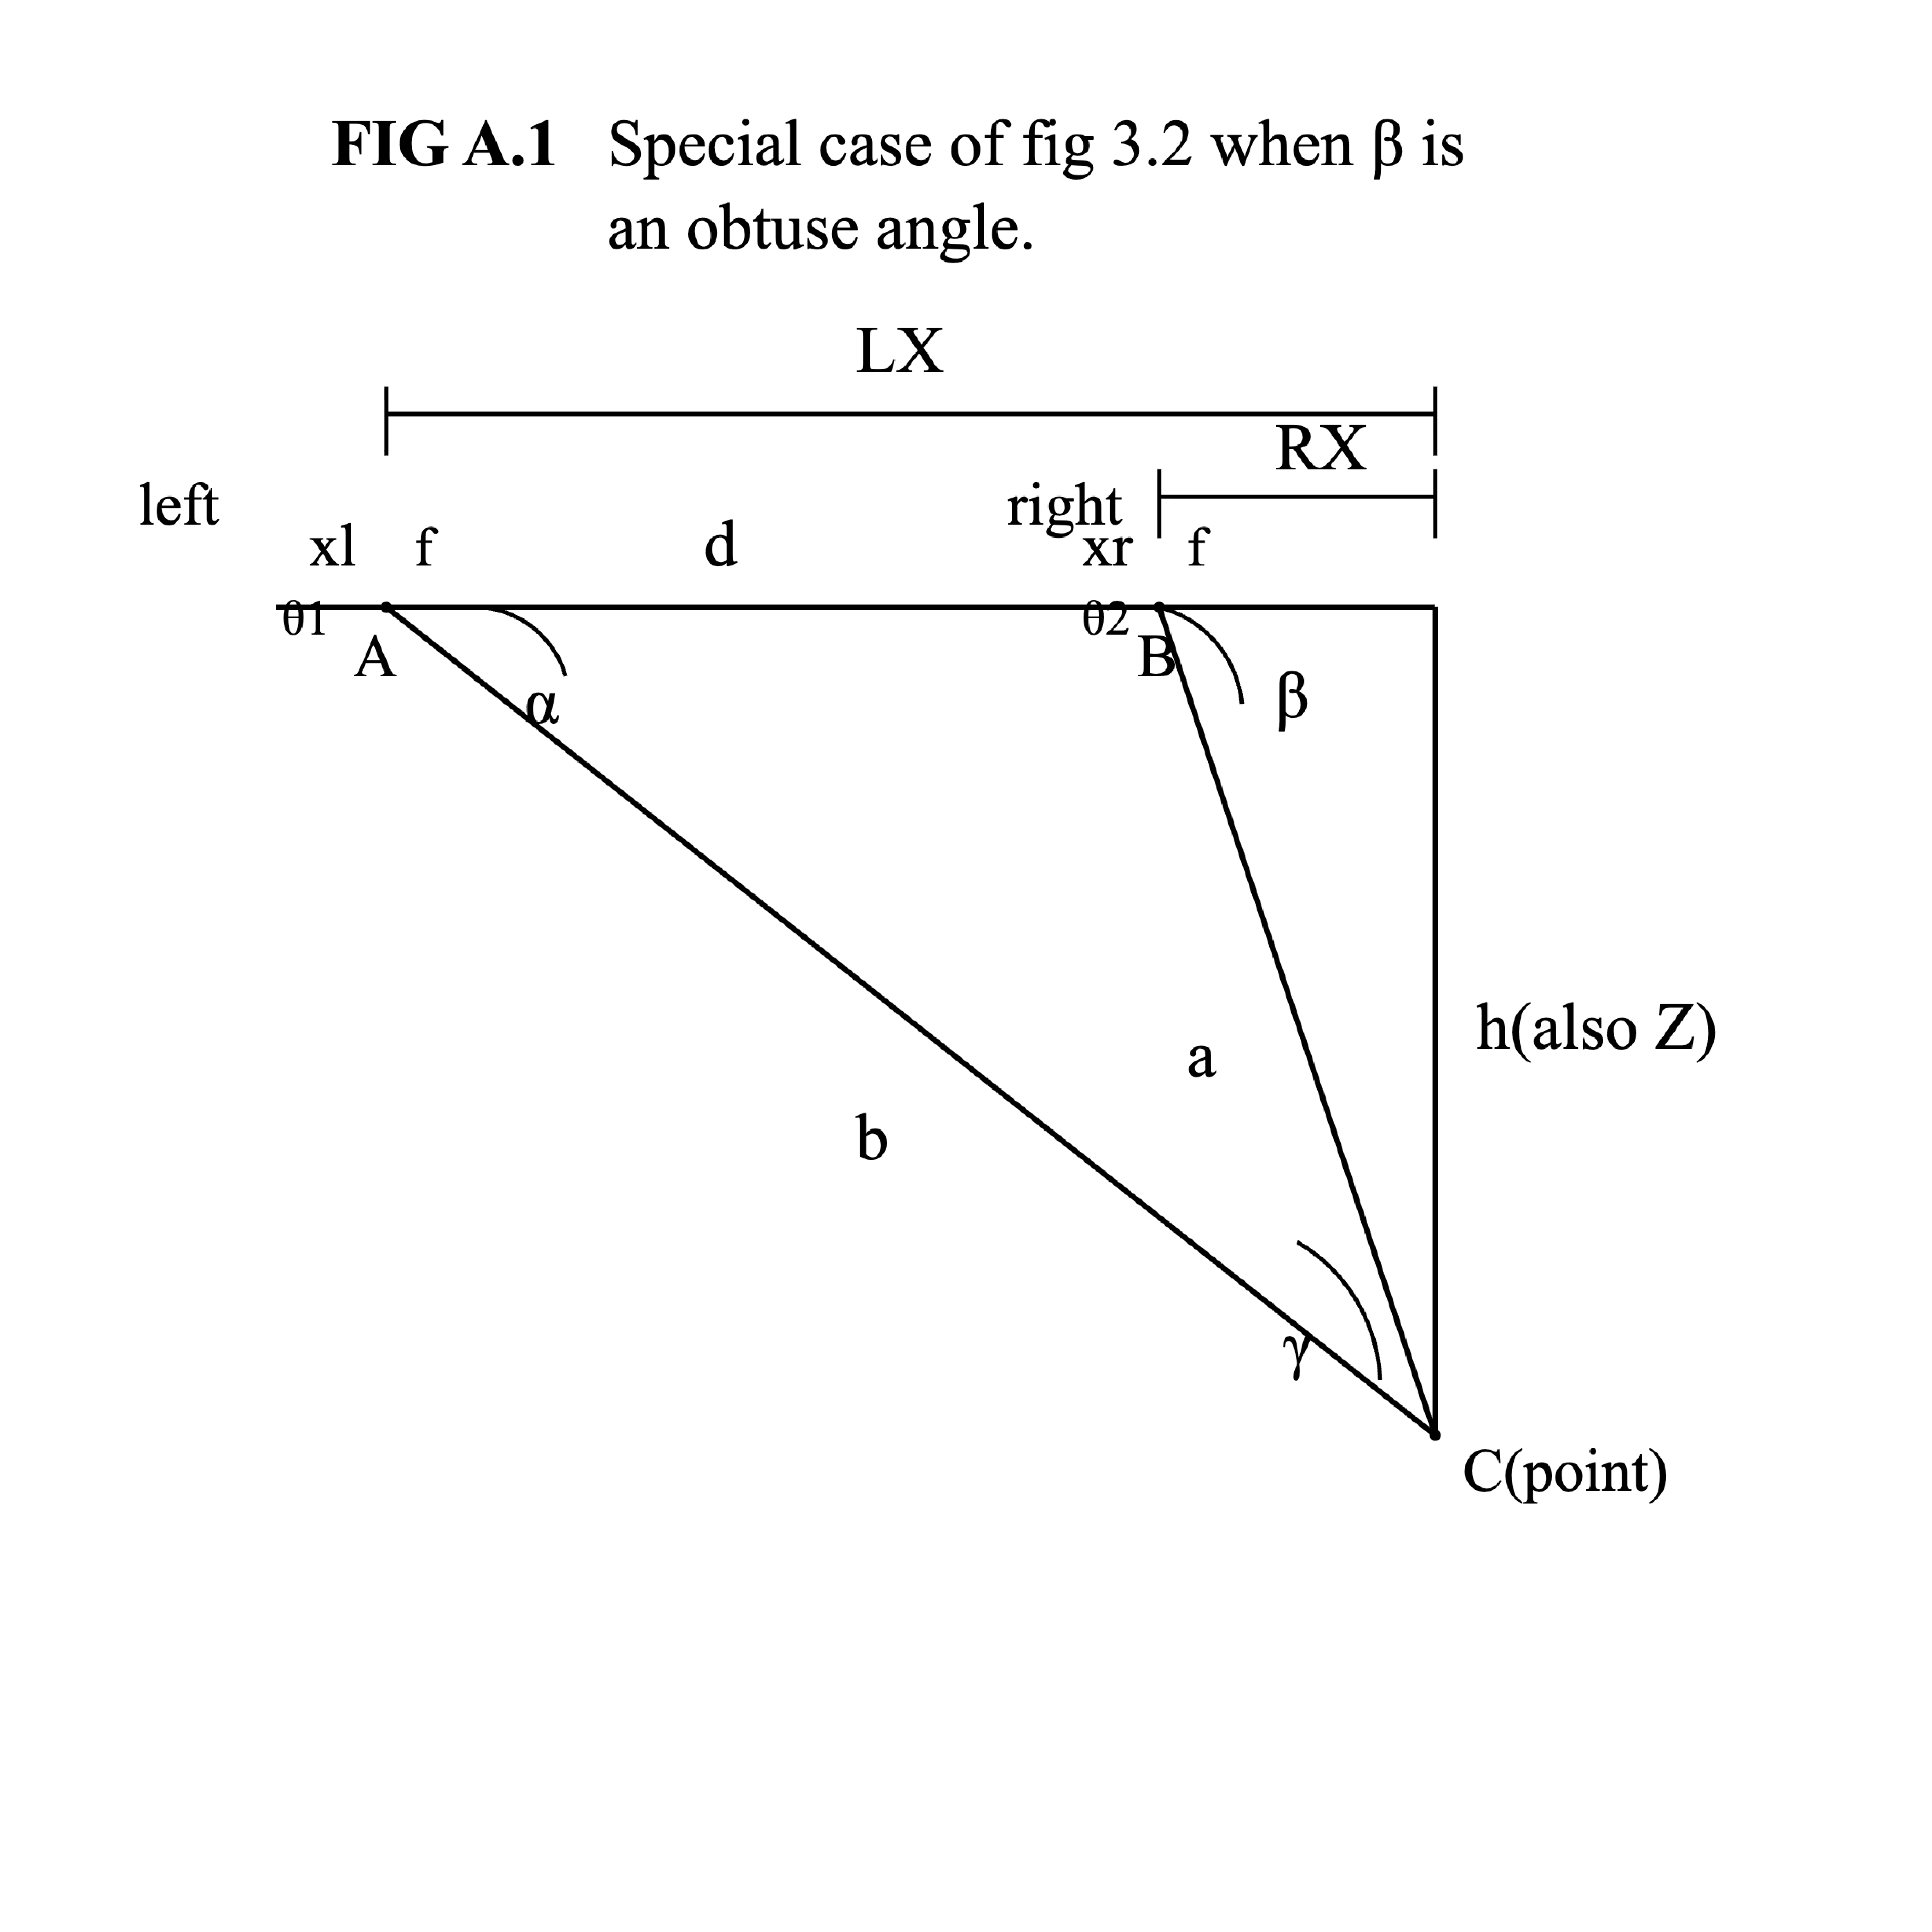
\includegraphics[width=0.8\textwidth]{appendix-1.pdf}
\caption{Representation of point falling on two negatives} 
\label{fig:stereo_negatives} 
\end{figure}
\section*{APPENDIX B} \textbf{Proof for the equality (3.6) for all types of triangles} \vspace{0.5cm} See Fig.~A.1 \begin{align} \frac{\sin\alpha}{a} &= \frac{h}{ba} \tag{A.1} \\[4mm] \frac{\sin\beta}{b} &= \frac{h}{ba} \tag{A.2} \end{align} \begin{align} \frac{\sin\gamma}{d} &= \frac{\sin[180^\circ-(\alpha+\beta)]}{d} \\[2mm] &= \frac{\sin(\alpha+\beta)}{d} \\[2mm] &= \frac{\sin\alpha\cos\beta+\cos\alpha\sin\beta}{d} \\[2mm] &= \frac{\left(\frac{h}{b}\right)\left(\frac{lx}{a}\right) + \left(\frac{lx}{b}\right)\left(\frac{h}{a}\right)} {lx+rx} \\[2mm] &= \frac{h(lx+rx)} {ba(lx+rx)} \\[2mm] &= \frac{h}{ba} \tag{A.3} \end{align} So, \[ \text{A.1} = \text{A.2} = \text{A.3} \] without imposing any conditions. Therefore equality (3.6), \begin{equation} \frac{\sin\alpha}{a} = \frac{\sin\beta}{b} = \frac{\sin\gamma}{d} \tag{3.6} \end{equation} holds true for any type of triangle.


\section*{APPENDIX C} \textbf{Proof for the equality (3.6) if in $\triangle ABC$ angle $\beta$ becomes an obtuse angle. The same treatment can be given for $\alpha$ if it becomes obtuse.} \vspace{0.3cm} See Fig.~A.1 \begin{align} \frac{\sin\alpha}{a} &= \frac{h}{b}\cdot\frac{1}{a} = \frac{h}{ba} \tag{A.1} \\[4mm] \frac{\sin\beta}{b} &= \frac{h}{a}\cdot\frac{1}{b} = \frac{h}{ba} \tag{A.2} \end{align} \begin{align} \gamma &= 180^\circ-\left(\alpha+\left(180^\circ-\beta\right)\right) \\ &= 180^\circ-\alpha-180^\circ+\beta \\ &= \beta-\alpha \end{align} \begin{align} \frac{\sin\gamma}{d} &= \frac{\sin(\beta-\alpha)}{d} \\[2mm] &= \frac{\sin\beta\cos\alpha- \cos\beta\sin\alpha}{d} \\[2mm] &= \frac{ \left(\frac{h}{a}\right)\left(\frac{lx}{b}\right) - \left(\frac{h}{b}\right)\left(\frac{rx}{a}\right)} {lx-rx} \\[2mm] &= \frac{h(lx-rx)} {ba(lx-rx)} \\[2mm] &= \frac{h}{ba} \tag{A.3} \end{align} Therefore, \[ \text{A.1} = \text{A.2} = \text{A.3} = \frac{h}{ba} \] Hence the equality (3.6), \begin{equation} \frac{\sin\alpha}{a} = \frac{\sin\beta}{b} = \frac{\sin\gamma}{d}, \tag{3.6} \end{equation} holds true.




 \end{document}